\documentclass{beamer}
\mode<presentation>
\usepackage{amsmath}
\usepackage{amssymb}
%\usepackage{advdate}
\usepackage{adjustbox}
\usepackage{subcaption}
\usepackage{enumitem}
\usepackage{multicol}
\usepackage{listings}
\usepackage{url}
\def\UrlBreaks{\do\/\do-}
\usetheme{Boadilla}
\usecolortheme{lily}
\setbeamertemplate{footline}
{
  \leavevmode%
  \hbox{%
  \begin{beamercolorbox}[wd=\paperwidth,ht=2.25ex,dp=1ex,right]{author in head/foot}%
    \insertframenumber{} / \inserttotalframenumber\hspace*{2ex} 
  \end{beamercolorbox}}%
  \vskip0pt%
}
\setbeamertemplate{navigation symbols}{}

\providecommand{\nCr}[2]{\,^{#1}C_{#2}} % nCr
\providecommand{\nPr}[2]{\,^{#1}P_{#2}} % nPr
\providecommand{\mbf}{\mathbf}
\providecommand{\pr}[1]{\ensuremath{\Pr\left(#1\right)}}
\providecommand{\qfunc}[1]{\ensuremath{Q\left(#1\right)}}
\providecommand{\sbrak}[1]{\ensuremath{{}\left[#1\right]}}
\providecommand{\lsbrak}[1]{\ensuremath{{}\left[#1\right.}}
\providecommand{\rsbrak}[1]{\ensuremath{{}\left.#1\right]}}
\providecommand{\brak}[1]{\ensuremath{\left(#1\right)}}
\providecommand{\lbrak}[1]{\ensuremath{\left(#1\right.}}
\providecommand{\rbrak}[1]{\ensuremath{\left.#1\right)}}
\providecommand{\cbrak}[1]{\ensuremath{\left\{#1\right\}}}
\providecommand{\lcbrak}[1]{\ensuremath{\left\{#1\right.}}
\providecommand{\rcbrak}[1]{\ensuremath{\left.#1\right\}}}
\theoremstyle{remark}
\newtheorem{rem}{Remark}
\newcommand{\sgn}{\mathop{\mathrm{sgn}}}
\providecommand{\abs}[1]{\left\vert#1\right\vert}
\providecommand{\res}[1]{\Res\displaylimits_{#1}} 
\providecommand{\norm}[1]{\lVert#1\rVert}
\providecommand{\mtx}[1]{\mathbf{#1}}
\providecommand{\mean}[1]{E\left[ #1 \right]}
\providecommand{\fourier}{\overset{\mathcal{F}}{ \rightleftharpoons}}
%\providecommand{\hilbert}{\overset{\mathcal{H}}{ \rightleftharpoons}}
\providecommand{\system}{\overset{\mathcal{H}}{ \longleftrightarrow}}
	%\newcommand{\solution}[2]{\textbf{Solution:}{#1}}
%\newcommand{\solution}{\noindent \textbf{Solution: }}
\providecommand{\dec}[2]{\ensuremath{\overset{#1}{\underset{#2}{\gtrless}}}}
\newcommand{\myvec}[1]{\ensuremath{\begin{pmatrix}#1\end{pmatrix}}}
\let\vec\mathbf

\lstset{
%language=C,
frame=single, 
breaklines=true,
columns=fullflexible
}

\numberwithin{equation}{section}

\title{10.4.3.1.3}
\author{Prajwal \\ EE24BTECH11051}
\begin{document}

\begin{frame}
\titlepage
\end{frame}
\section*{Outline}
\begin{frame}
\tableofcontents
\end{frame}
\section{Problem}
\begin{frame}
\frametitle{Problem Statement}
Find the roots of the following quadratic equations by completing the squares if exits.
\end{frame}
%\subsection{Literature}
\section{Solution}
\subsection{Theoretical Solution}
\begin{frame}
\frametitle{Theoretical Solution}
    Checking roots of equation exist or not,

    \begin{align}
    b^2 - 4ac \geq 0 \\
    = 48 - 4(4)(3)\\
    = 0 
    \end{align}
    This means roots of equation exist and are coincident.\\
    And its root is given by 
    \begin{align}
    4x^2 + 4\sqrt{3}x + 3 = 0 \\
    (2x-\sqrt{3})^2 = 0 \\
    x = -\frac{\sqrt{3}}{2}=-0.866025
    \end{align} 
\end{frame}
\section{Computational logic}
\begin{frame}[fragile]
    \frametitle{Computational logic}
    \textbf{Eigen value method}
    
    \item Characteristics polynomial is given by
    \begin{align}
     p(x)=a_nx^n+a_{n-1}x^{n-1}+\cdots +a_1x+a_0   
    \end{align}
    where $a_n \neq 0$
    \item Divide Characteristics equation by $a_n$
    \begin{align}
        p(x)= a_nx^n+a_{n-1}x^{n-1}+\cdots +a_1x+a_0     \\
        p(x)=x^n+\frac{a_{n-1}}{a_n}x^{n-1}+\cdots +\frac{a_1}{a_n}x+\frac{a_0}{a_n}
    \end{align}
    \item Companion Matrix of characteristic polynomial is given by:\\
    Let
    \begin{align}
        \begin{bmatrix}
        0 & 1 & 0 & \cdots & 0 \\
        0 & 0 & 1 & \cdots & 0 \\
        \vdots & \vdots & \vdots & \ddots & \vdots \\
        0 & 0 & 0 & \cdots & 1 \\
        -\frac{a_0}{a_n} & -\frac{a_1}{a_n} & -\frac{a_2}{a_n} & \cdots & -\frac{a_{n-1}}{a_n}
    \end{bmatrix}
    \end{align}
\end{frame}
\begin{frame}[fragile]
    \item QR decomposition 
    \begin{align}
    A = QR
    \end{align}
    \item $Q$ is an $ m \times n $ orthogonal matrix
    \item $R$ is an $n \times n$ upper triangular matrix.
    Given a matrix $ A = [a_1, a_2, \dots, a_n] $, where each $ a_i $ is a column vector of size $ m \times 1 $.

    \item Normalize the first column of $A$:
    \begin{align}
    q_1 = \frac{a_1}{\norm{a_1}}
    \end{align}
    
    \item  For each subsequent column $ a_i $, subtract the projections of the previously obtained orthonormal vectors from $ a_i $ :
    \begin{align}
    a_i' = a_i - \sum_{k=1}^{i-1} \langle a_i, q_k \rangle q_k
    \end{align}
    Normalize the result to obtain the next column of \( Q \):
    \begin{align}
    q_i = \frac{a_i'}{\norm{a_i'}}
    \end{align}
\end{frame}
\begin{frame}[fragile]
    Repeat this process for all columns of \( A \).
    \item Finding $R$:- \\
    After constructing the ortho-normal columns $ q_1, q_2, \dots, q_n $ of $Q$, we can compute the elements of $R$ by taking the dot product of the original columns of $A$ with the columns of $Q$:
    \begin{align}
    r_{ij} = \langle a_j, q_i \rangle \text{ , for  }  i \leq j 
    \end{align}
    \item \textbf{QR-Algorithm}\\
    \item Initialization \\
    Let $A_0 = A $, where $A$ is the given matrix.
    \item QR Decomposition \\
For each iteration $ k = 0, 1, 2, \dots $:
    \item Compute the QR decomposition of \( A_k \), such that:
    \begin{align}
    A_k = Q_k R_k
    \end{align}
    where:
        \item $Q_k $ is an orthogonal matrix ($ Q_k^\top Q_k = I $).
        \item $ R_k $ is an upper triangular matrix.
    The decomposition ensures $ A_k = Q_k R_k $.

\end{frame}
\begin{frame}[fragile]
        \item Form the next matrix \( A_{k+1} \) as:
    \begin{align}
    A_{k+1} = R_k Q_k
    \end{align}
\item Convergence\\
Repeat Step 2 until $ A_k $ converges to an upper triangular matrix $ T $. The diagonal entries of $T$ are the eigenvalues of $A$.\\
\item The eigenvalues of matrix will be the roots of the equation.
\end{frame}
\begin{frame}[fragile]
    \begin{figure}[h]
    \centering
    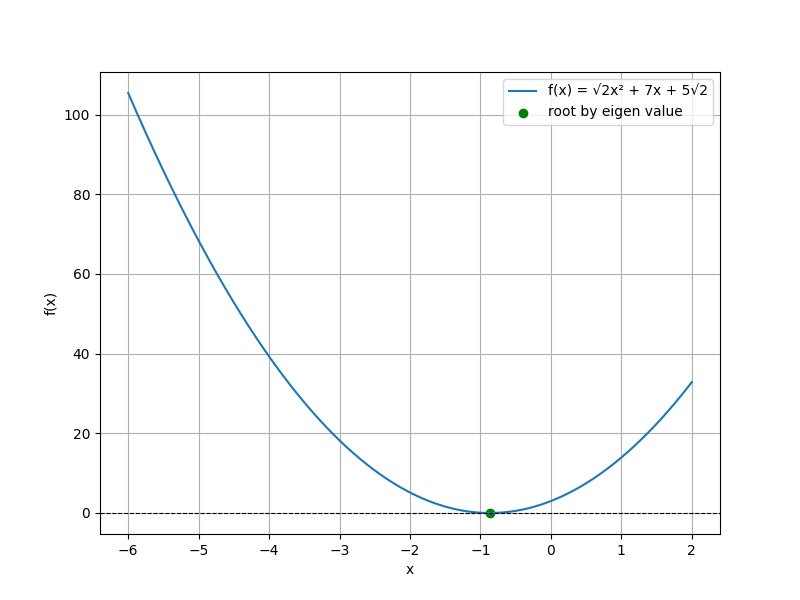
\includegraphics[width=\columnwidth]{figs/fig.png}
 \end{figure}
\end{frame}
\end{document}
